\section{Motivation}
Recently, various studies are proposed to exploit the stream feature.
First, Kang et al.~\cite{MultiStream} proposed that the application
is modified to manually assign streams.
Since an application knows the lifetime of the data best, this approach
is very effective in reducing WAF.
However, in order to properly specify streams in the application, the programmer must
fully understand the lifetime characteristics of data.
Also when multiple applications try to assign streams, a centralized stream assignment
is required to avoid conflicts.
Second, FStream~\cite{FStream} separates short-lived data, e.g., file system metadata and
journal, using the file system information. 
FStream does not require a burden on the programmer, but the system developer is still burdened
to identify short-lived data of the application, e.g., log data of key-value store, based on the file extension.
Lastly, unlike other scheme, AutoStream~\cite{AutoStream} is aimed to automate the process of mapping 
write I/O operations to an SSD stream.
Since AutoStream relies on the past LBA access patterns, it is not practical when the data are written in
append-only manner, as modern key-value store.

We analyzed RocksDB~\cite{RocksDB}, one of the popular key-value store, 

\begin{figure}[!t]
	\centering
	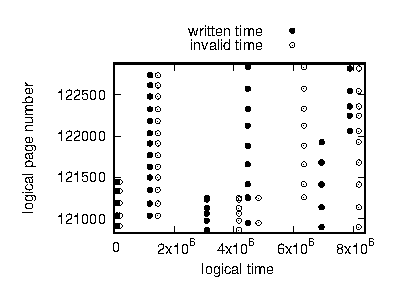
\includegraphics[width=0.9\linewidth]{figure/chunklifetime} % data from 1/02271857 - 59 chunk 
	\caption{The various lifetime of data of append-only workload with in a chunk}
	\label{fig:chunklifetime}
\end{figure}

Summarizing existing studies, if we adopt automated stream management to the append-only workload,
we lose the lifetime information of the application. 


